\documentclass{jsarticle}
\usepackage{multicol}

% sourcecode highlight
\usepackage{color}
\usepackage{listings,jlisting}

%jlisting (sourcecode highlight)
\lstset{
language={C},
backgroundcolor={\color[gray]{.85}},
basicstyle={\small},
identifierstyle={\small},
commentstyle={\small\ttfamily \color[rgb]{0,0.5,0}},
keywordstyle={\small \color[rgb]{0,0,0}},
ndkeywordstyle={\small},
stringstyle={\small\ttfamily \color[rgb]{0,0,1}},
frame={tb},
breaklines=true,
columns=[l]{fullflexible},
numbers=left,
xrightmargin=0zw,
xleftmargin=3zw,
numberstyle={\scriptsize},
stepnumber=1,
numbersep=1zw,
morecomment=[l]{//}
}

%comment out multiple line
\usepackage{comment}

%image
\usepackage[dvipdfmx]{graphicx}
\usepackage{here}


\title{麻雀点数計算プログラム\ 注釈書}
\author{14EC004\ 飯田頌平}

\begin{document}
\maketitle

\begin{multicols}{2}

\section{はじめに}
本稿は吉田さんの麻雀点数計算プログラム\cite{yoshida}
の注釈書にあたる。

このプログラムはカメラで麻雀の手牌を撮影すると
点数を自動で計算するというものであり、
大まかにサーバ、画像認識、点数計算の三つのモジュールに分かれている。

このうち本稿では画像認識の部分について触れる。
画像認識の実装ファイルTemplateMatching.scala
およびユーザ定義関数の実装ファイルpackage.scala
を付録に掲載するので、参考にしながら読むこと。

\section{プログラムの実行方法}

プログラムはgithub上に上げられているが、
それをcloneするだけでは動作しない。
sbtをインストールした上で、opencvを使用できるようにせねばならない。

Ubuntuであれば、sbtは以下のコマンドでインストールできる。
\begin{lstlisting}[caption=sbt,label=sbt]
$ sudo apt-get install sbt
\end{lstlisting}

opencvは各自自力でコンパイルする必要がある。
公式ドキュメントを参考にして、以下のコマンドを実行して.soファイルを生成する。
\begin{lstlisting}[caption=opencv,label=opencv]
$ git clone git://github.com/Itseez/opencv.git
$ cd opencv
$ mkdir build
$ cd build
$ cmake -DBUILD_SHARED_LIBS=OFF
$ make -j8
\end{lstlisting}

.soファイルはopencv/build/libに生成されるはずである。
もし生成されていない場合は、cmakeの出力結果を確認すること。
To\ be\ builtの項目にjavaとない場合は、java-8-oracleの環境変数を設定できていないので、
\begin{lstlisting}[caption=JAVAHOME,label=j]
$ JAVA_HOME=/usr/lib/jvm/java-8-oracle
\end{lstlisting}
を実行すること。

生成された.soファイルを、cloneしてきたmahjongsディレクトリの下の
mahjongs/recogniser/lib
に置けばsbt環境下でopencvを使用することができるようになる。

\section{画像認識のフロー}

画像認識はパターンマッチングによって行われている。
よって、最初にテンプレートを生成し、その後テストデータとテンプレートを照合させて結果を求める。
まずはテンプレートの生成手順を示す。
\begin{enumerate}
\item 雀牌を黒と白で二値化する
\item 雀牌の輪郭を判別し、雀牌だけを切り取る
\item 雀牌から牌ひとつあたりの縦幅と横幅を求める
\item 黒と判別された誤差(牌の隅)を白く塗りつぶす
\item 牌の絵柄部分の輪郭情報を得る
\item 輪郭情報と雀牌のグレースケール画像からテンプレートを生成する
\end{enumerate}

詳細な説明については後述するとして、
次に照合の手順を示す。
\begin{enumerate}
\item 手牌の輪郭を判別し、手牌(純手牌+鳴牌)だけを切り取る
\item テンプレートと同じサイズにリサイズする
\item 取得した輪郭の頂点数を求める(四角形なら純手牌である)
\item テンプレートから各牌を回転させたイメージを得る
\item 手牌とテンプレート(及び回転イメージ)をテンプレートマッチングで照合する
\item 照合結果に牌種のシーケンスを与え、結果の最大スコアを取り出す
\item 最大スコアを基に矩形を作成し、手牌を矩形領域で塗りつぶす
\item 5.6.7.の手順を再帰的に繰り返すと、手牌が黒く塗りつぶされてゆく。
		  完全に塗りつぶされたら、再帰を終了する
\item 純手牌を第一要素、鳴牌を第二要素のタプルを作り、関数の結果として返す
\end{enumerate}

こうして手牌を認識することができた。
次章以降ではこれらの流れの詳細について述べる。

\section{テンプレートの生成}

テンプレートの生成にあたって、
まずは元画像を用意する。
以下にその要件を示す。
\begin{itemize}
\item 雀牌を4*9の矩形上に隙間なく並べる。矩形は平行になるようにする
\item 牌の位置は固定である。
		  一萬からはじまるSEQが予め定められている
\item 雀牌と背景以外のものを除外する
\item 撮影時に、各牌が等しい高さと幅を持つよう注意する
\item 二値化からの境界値探索を阻害しないよう背景を選ぶ
\end{itemize}

背景には麻雀マットなどを用いれば良い。
また斜めから撮影された画像からは正しいテンプレートが得られないことに気を付ける。

実際に使用したテンプレート画像を図\ref{fig:template}に示す。

\begin{figure}[H]
  \begin{center}
    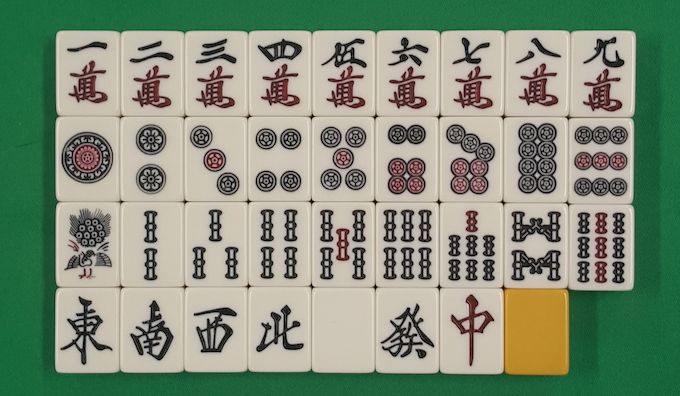
\includegraphics[clip,width=7.0cm]{./img/template.png}
    \caption{テンプレート}
    \label{fig:template}
  \end{center}
\end{figure}

この画像の画素値は幅680x高さ396ピクセルであり、
ビットの深さは32である。
このビット数はグレースケール変換後(図\ref{fig:templateGray})には8ビットまで圧縮される。

\begin{figure}[H]
  \begin{center}
    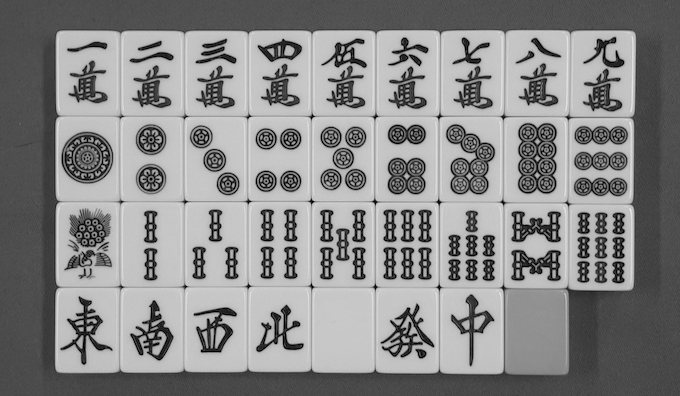
\includegraphics[clip,width=7.0cm]{./img/template_gray.png}
    \caption{テンプレート\ グレースケール}
    \label{fig:templateGray}
  \end{center}
\end{figure}

元画像は図\ref{fig:templateGray}の状態に変換された後にプログラムへMat型で渡される。
Mat型はopencv\footnote{https://github.com/bytedeco/javacv}のライブラリが提供する行列の型であり、
opencvではこの型で画像データを扱う。
Mat型の内部構造は行列、画素値、画素のデータ型である。
createTemplateの引数matが元画像のデータを示す変数である。

matに対して最初に行われる処理は、定数MaxResolutionのサイズに近づくよう
resizeで画像サイズを修正する。
大きい画像であると処理時間が増えてしまうため、これによって効率化する。

次に雀牌と背景を識別し、雀牌だけを切り取るcropを実行する。
cropは元画像を引数に取り、Buffer型のシーケンスで識別結果の画像を返す。
(なおBufferはタプルであり、画像だけでなく輪郭の二次元配列も返しているが、
この値はcreateTemplateでは参照しない。)

cropの実装は、
まずfindContoursによって元画像を輪郭で分離し、
minAreaRectで矩形を得て、
warpAffineで矩形の傾きを底面と垂直になるよう修正し、
getRectSubPixで矩形領域のピクセル値を得ることで、
入力画像を輪郭毎に分離した上で補正をかけた画像を得るようになっている。

輪郭を切り取る関数findContoursの理論を示す。
\begin{enumerate}
\item 二値化を行う
\item 画素の左上から右下にかけて白の値を走査する
\item 白の値が見つかれば、そこを基点と定める
\item 基点に隣接する白の値を探し、見つかればそこを新たな基点として再帰的に輪郭を得る。
		  見つからなければ孤立点または孤立線として捉え、輪郭を抽出できたとする
\item 最初の基点と現在の基点が重なったときに、輪郭を抽出出来たとする
\item すべての画素の走査が終了するまで2.~5.を繰り返す
\end{enumerate}

当プログラムでは最も高いヒエラルキーの輪郭のみを抽出しているため、処理が高速である。
ヒエラルキーとはopencvの概念であり、輪郭の内部にまた別の輪郭がある場合、後者は前者の子だとして階層関係を定義しているのだが、
ここでは子となるあらゆる輪郭を無視している。

findContoursの実装についてはドキュメントに数式が散見されず、
またソースコード(contours.cpp)が1700行にも上る\cite{contours}ため、
解析は困難であった。
代わりに上述の理論に基づいたアルゴリズムを自分で実装したので、
そのようなアルゴリズムが使われていたのだと仮定することにする。
実装したアルゴリズムを以下に示す。

\end{multicols}

\begin{lstlisting}[caption=輪郭抽出アルゴリズム,label=contour]
import cv2

class boader:

  base = {"row": 0, "col": 0}
  isolate = []

  def threshold(self, img):
    res = img
    for y in range(len(img)):
      for x in range(len(img[y])):
        if img[y][x] >= 128:
          buf = 255
        else:
          buf = 0
        res[y][x] = buf
    return res

  def directions(self, n):
    """
    When recursiving, send index of direction.
    Right-back direction is gotten by (n+4+1) % 8
    """
    if n==0:
      direction = [[-1,-1], [0,-1], [1,-1], [1,0], [1,1], [0,1], [-1,1], [-1,0]]
    elif n==1:
      direction = [[0,-1], [1,-1], [1,0], [1,1], [0,1], [-1,1], [-1,0], [-1,-1]]
    elif n==2:
      direction = [[1,-1], [1,0], [1,1], [0,1], [-1,1], [-1,0], [-1,-1], [0,-1]]
    elif n==3:
      direction = [[1,0], [1,1], [0,1], [-1,1], [-1,0], [-1,-1], [0,-1], [1,-1]]
    elif n==4:
      direction = [[1,1], [0,1], [-1,1], [-1,0], [-1,-1], [0,-1], [1,-1], [1,0]]
    elif n==5:
      direction = [[0,1], [-1,1], [-1,0], [-1,-1], [0,-1], [1,-1], [1,0], [1,1]]
    elif n==6:
      direction = [[-1,1], [-1,0], [-1,-1], [0,-1], [1,-1], [1,0], [1,1], [0,1]]
    elif n==7:
      direction = [[-1,0], [-1,-1], [0,-1], [1,-1], [1,0], [1,1], [0,1], [-1,0]]
    else:
      print("directions catch undefined number as parameter:" + str(n))
    return direction

  def directionDecoder(self, y, x):
    # getting forward direction
    n = 0
    if x==-1:
      if y==-1: n = 0
      elif y==0: n = 1
      elif y==1: n = 2
    elif x==0:
      if y==-1: n = 7
      elif y==1: n = 3
    elif x==1:
      if y==-1: n = 6
      elif y==0: n = 5
      elif y==1: n = 4
    res = (n+5)%8
    print("res:" + str(res) + ", y:" + str(y) + ", x:" + str(x))
    return res

  def recursiveSearch(self, img, row, col, contour, directionNum):
    """
    1. base-point is passed as parameter
    2. search black-point using counterclockwise rotation.
       start direction is right-back
    3. if find black-point, deciding direction and recursiving and fill new black-point marker number "1". marker number is reseted on going to new base-point
       if not find black-point, back previous point and search another point
    4. if reach base-point, contour extraction is finished
    """

    # 8 direction (Northwest -> West -> ... -> North)
    direction = self.directions(directionNum)
    print("-" * 30)
    print("row:" + str(row) + ", col:" + str(col))
    print("directionNum:" + str(directionNum))
    print("direction:")
    print direction

    for i in range(len(direction)-1):
      y = row + direction[i][0]
      x = col + direction[i][1]

      # only permit number can be in index
      if (y >= 0 and y < len(img)) and (x >= 0 and y < len(img[y])): 
        if len(contour) > 30: #forcely finish(for debug)
            b += 0
        # if find black-point
        if img[y][x]==0:
          # if black-point is base-point
          if y==self.base["row"] and x==self.base["col"]:
            img[y][x] = 1 # fill
            return (contour, True) # back to recursiving-parent
          else:
            newDirectionNum = self.directionDecoder(direction[i][0], direction[i][1])
            img[y][x] = newDirectionNum+10 # fill (for duplication)
            c = contour
            c.append([y, x])
            print("direction=>[y, x]:", str(direction[i][0]) + ", " + str(direction[i][1]))
            res = self.recursiveSearch(img, y, x, c, newDirectionNum)
            if res[1] == True:
              self.isolate = [] # reset
              return res # back to searchBoader

    # if not found new black-point
    """
    1. traceback previous point
    2. check new black-point(without deadend route)
       deadend route is ignored by fill
    3. if traceback reach base-point, this case is getting curve
    4. in other case, when isolate curve is detected, use global variable "isolate" and assign deadend-contour. "isolate" is final variable, re-assignment is only permitted in end of recursiving for reset
    """
    if len(self.isolate) == 0:
      self.isolate = contour
    if len(self.isolate)==1 or row==self.base["row"] and col==self.base["col"] :
      img[y][x] = 1 # fill
      isl = self.isolate
      self.isolate = []
      return (isl, True) # back to recursiving-parent
    c = contour[:-1]
    res = self.recursiveSearch(img, contour[len(contour)-1][0], contour[len(contour)-1][1], c, 0) # in this case, black-point duplication is not found. then, directionNum is any value.
    if res[1] == True:
      self.isolate = []
      return res

    print("contour::False")
    self.isolate = []
    return (contour, False)

  def searchBoader(self, img):
    """search most external contour."""
    res = []
    img = b.threshold(img)
    for y in range(len(img)):
      for x in range(len(img[y])):
        if img[y][x] == 0:
          self.base["row"] = y
          self.base["col"] = x
          buf = self.recursiveSearch(img, y, x, [[y, x]], 0)
          if buf[1]==True:
            res.append(buf[0])
            img = self.fill(img, buf[0])

    self.show(img)
    return res

  def show(self, img):
    print img

  def fill(self, img, contour):
    """
    fill inner contour.
    in case, fill make black pixel inner contoutr assign value of 2.
    because black pixel referenced by searchBoader is only value of 0.
    """
    fillVal = 2
    whiteVal = 255
    flag = 0
    for c in contour:
      img[c[0]][c[1]] = fillVal
    for y in range(len(img)):
      prev = whiteVal # prev is used for detecting edge
      for x in range(len(img[y])):
        if not img[y][x] == prev:
          if prev > img[y][x]: flag = 1
          else: flag = 0
        if flag == 1: img[y][x] = fillVal
        prev = img[y][x]

    return img


b = boader()
img = cv2.imread("zero.jpg", 0)
res = b.searchBoader(cv2.resize(img, (10, 10)))
print res
\end{lstlisting}

\begin{multicols}{2}

このアルゴリズムでは次の基準点を探すときに方向を取得しており、
移動方向から右斜め後ろにあたる点から反時計回りの順で画素の輝度を探索するようにしている。
%内側の判定(複数の輪郭が重なるケース)が未完成のコード。最外殻のみ取れる

このアルゴリズムについて図\ref{fig:zero}で実験を行ったところ、
図\ref{fig:zeroRes}のような結果が得られた。
出力されたリストを見れば、輪郭を抽出できていることがわかる。

\begin{figure}[H]
  \begin{center}
    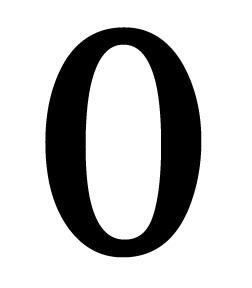
\includegraphics[clip,width=3.0cm]{./img/zero.png}
    \caption{輪郭抽出実験\ 元画像}
    \label{fig:zero}
  \end{center}
\end{figure}

\begin{figure}[H]
  \begin{center}
    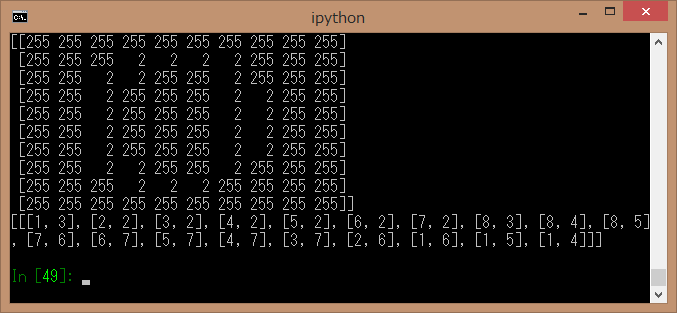
\includegraphics[clip,width=7.0cm]{./img/zeroRes.png}
    \caption{輪郭抽出実験\ 結果}
    \label{fig:zeroRes}
  \end{center}
\end{figure}

麻雀認識プログラムの輪郭抽出の話に戻るが、
最終的に、図\ref{fig:templateContour}のように輪郭が取得される。

\begin{figure}[H]
  \begin{center}
    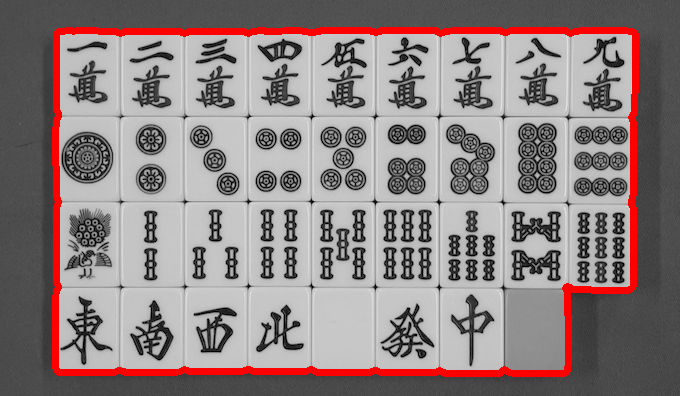
\includegraphics[clip,width=7.0cm]{./img/template_contour.png}
    \caption{テンプレート\ 輪郭}
    \label{fig:templateContour}
  \end{center}
\end{figure}

opencvの輪郭抽出メソッドfindCountoursから
得た輪郭countourのメソッドtoArrayを用いれば、
minAreaRectで矩形を引くべき座標を得られる。

こうして得られた分離後の画像のシーケンス(返り値はBuffer型であることに注意)から
headOptionを使うことで先頭要素を取り出せる。
findContoursを呼び出した際に大きさ順に画像をソートしているので、
先頭要素には一番大きな画像が入る。
一番大きな画像が雀牌であるという前提であるなら、
この先頭要素は雀牌であるため、雀牌のテンプレートは引数templateに束縛される。
findCountersは複数の輪郭を検出できたとき、それらをまとめて返すため、このようにして雀牌を取り出す。

以上の処理を行い輪郭抽出を終えた画像を図\ref{fig:templateCrop}に示す。

\begin{figure}[H]
  \begin{center}
    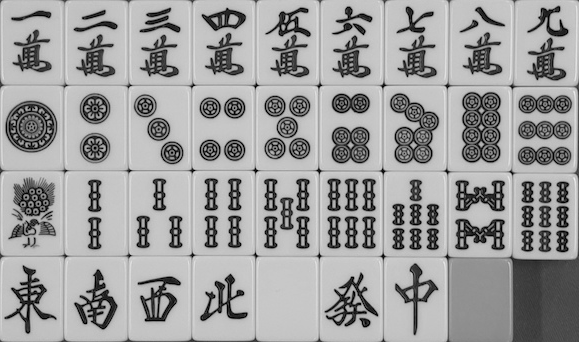
\includegraphics[clip,width=7.0cm]{./img/template_crop.png}
    \caption{テンプレート\ 輪郭抽出済}
    \label{fig:templateCrop}
  \end{center}
\end{figure}

得られた雀牌画像をthresholdによって黒と白で二値化すると、図\ref{fig:templateBinary}の様な画像になる。

\begin{figure}[H]
  \begin{center}
    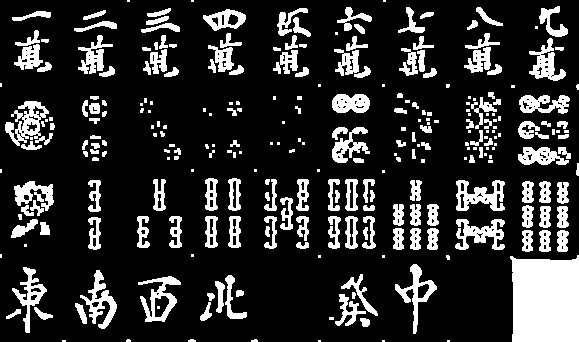
\includegraphics[clip,width=7.0cm]{./img/template_binary.png}
    \caption{テンプレート\ 二値化}
    \label{fig:templateBinary}
  \end{center}
\end{figure}

ここでは模様が白、牌の白地が黒に分離されている。
二値化処理では白地が白となるのが普通だが、ここでは二値化の後に反転をかけてあえて白地を黒、模様を白としている。
これはopencvの輪郭抽出処理が黒を背景として切り捨てるため\cite{contoursDoc}であり、
この後模様の輪郭抽出を行う際に模様を白くして抽出できるようにする。

二値化の閾値は大津の二値化と呼ばれるアルゴリズムを用い、統計的に自動で算出する。
大津の二値化について説明する。
まず横軸に輝度、縦軸に画素数を取ったヒストグラム(図\ref{fig:otsu})を画像データから生成する。

\begin{figure}[H]
  \begin{center}
    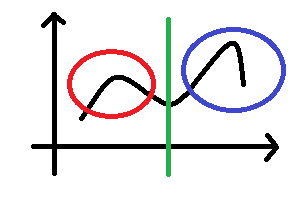
\includegraphics[clip,width=7.0cm]{./img/otsu.png}
    \caption{輝度-画素数のヒストグラム}
    \label{fig:otsu}
  \end{center}
\end{figure}

図中の赤い領域と青い領域をうまく分離できるような閾値(緑線)を探索することがこのアルゴリズムの目的である。

閾値を評価する指数として、分離度という値を導入する。
分離度はクラス内分散$σ_{w}$に反比例し、クラス間分散$σ_{b}$に比例する。
$σ_{w}$、$σ_{b}$はそれぞれ以下の式で表される。

\begin{eqnarray}
\label{sigmaw}
{ \sigma  }_{ w } & = & \frac { { w }_{ 1 }{{ \sigma  }_{ 1 }}^{2}+{ w }_{ 2 }{{ \sigma  }_{ 2 } }^{2}}{ { w }_{ 1 }+{ w }_{ 2 } } 
\end{eqnarray}

\begin{eqnarray}
\label{sigmab}
{ \sigma  }_{ b } & = & \frac { { w }_{ 1 }{{ \left( { m }_{ 1 }-{ m }_{ t } \right)  }}^{2}+{ w }_{ 2 }{\left( { m }_{ 2 }-{ m }_{ t } \right)}^{2}  }{ { w }_{ 1 }+{ w }_{ 2 } } 
\end{eqnarray}

クラス内分散とは各クラス(赤領域と青領域)についての分散を出し、各クラスのデータ数で重み付けをして求められる、
各クラス毎のまとまりを包括的に示す指標である。

一方クラス間分散とは全体の平均値と各クラスの平均値を使って求められる分散であり、
これは各クラスがどれだけ散らばっているのかを示す指標である。

最終的に分離度は、定数を切り離して

\begin{eqnarray}
\label{eq:sigma}
\sigma = w_{1} w_{2}{\left(m_{1}-m_2 \right)}^{2}
\end{eqnarray}

によって示される。式\ref{eq:sigma}が最大となる閾値を求めればよい。
輝度が8bitならば試行回数は256で済むので、総当りで探索しても差し支え無いだろう。

%
\begin{comment}
さて、ここまでで輪郭抽出と二値化を通し図\ref{fig:templateBinary}を得ることが出来た。
ここで図\ref{fig:templateBinary}の雀牌群データを分割し、雀牌ひとつあたりのデータにする。
widthとheightに牌ひとつあたりの幅と高さを代入する。
このとき雀牌の並びが4*9でなかったとき、想定外の値を取ってしまうので注意すること。
\end{comment}

こうして得られた二値化後の画像(図\ref{fig:templateBinary})について見てみると、
牌の模様が白、牌の背景が黒で表されているものの、
牌と牌の間なども白く判定されてしまっている。
牌の模様以外が白と認識されてはパターンマッチに失敗しやすくなるため、
次はこの誤判定部分を黒く塗りつぶす。
それにはfloodFillを使う。
floodFillは座標を指定し、連結部分を指定した色で塗りつぶす関数である。
これを牌と牌の間にすべてに対して実行することで、
誤判定が塗りつぶされる。

さらにfloodFillの補完として、dilateを使用する。
dilateは膨張処理によってノイズを消す効果があり、
ターゲットの周辺に1ピクセルでも白があれば、ターゲットを白に置き換える処理を行う。
これによって牌の模様をはっきりとさせる。

floodFillとdilateをかけた結果の画像を図\ref{fig:templateFill}に示す。
図\ref{fig:templateBinary}に比べると、牌と牌の間が塗りつぶされていることと、模様の部分が膨張していることがわかる。

\begin{figure}[H]
  \begin{center}
    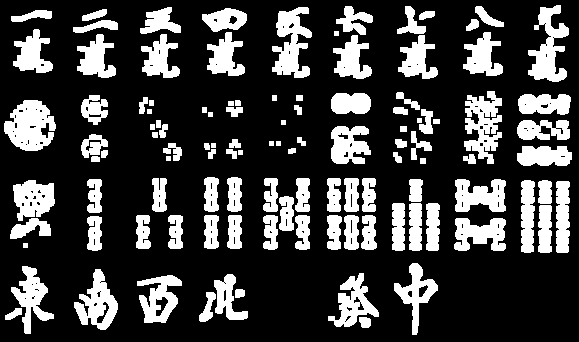
\includegraphics[clip,width=7.0cm]{./img/template_fill.png}
    \caption{塗りつぶし・膨張処理後}
    \label{fig:templateFill}
  \end{center}
\end{figure}

そして牌の模様だけを抽出する。
二値化した値に対してfindContoursによって再び輪郭ごとの分離をかければ、
模様だけを抽出することができる。
四筒のように模様が複数に分離されてしまうケース(二筒ふたつとして認識される)の場合は、
convexHullによって結合する。
convexHullは点群の凸包を得た後に外接する矩形で近似する。

凸包の近似のアルゴリズムを示す。
まずは基準点を決定する。
この際基準点となりうる点は、凸包を形成する点でなくてはならないので、
点集合の最も上部にある点を基準点とする。
この点を求めるには、画像の左上から右下にかけて走査し、
最初に当たった点を極地にある点だと見做せばよい。

次に基準点を始点とする半直線(基準線)を置く。
左上から右下への走査を行った場合は、画像に対し真上の方向か、それに左へ直角な基準線を考える。

そして基準点からあらゆる他の点集合に対して直線を引き、
その直線と基準線との角度の差が最も小さい点が、凸包を形成する点であると見なせる。

後は再帰的にこれまでの処理を繰り返し、多角形が形成されれば凸包を求めることができる。

%
%sklansky法
%
\begin{comment}
opencvのconvexHullはSklanskyのアルゴリズムによって凸法を求めている。
そのアルゴリズムの流れを示す。

まずは凸法を求めたい点集合を用意する。
そして上下左右四方向の極地の点を取得し、点T,B,L,Rとする。
点T,B,L,Rより四角形を作り、その四角形に外接する矩形を描く(図\ref{fig:sklansky1})。

\begin{figure}[H]
  \begin{center}
    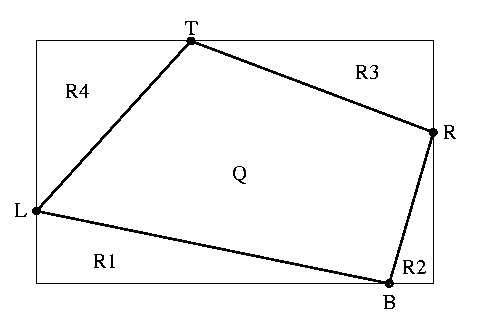
\includegraphics[clip,width=7.0cm]{./img/sklansky1.png}
    \caption{Sklansky法-外接矩形の作成}
    \label{fig:sklansky1}
	 {\tiny http://cgm.cs.mcgill.ca/~athens/cs601/}
  \end{center}
\end{figure}

R1領域について考える。
Lを凸包の頂点Iとし、
Iを始点とする直線上に凸包の頂点I+1を置くと、それはR1領域を図(\ref{fig:sklansky2})のように分割する。

\begin{figure}[H]
  \begin{center}
    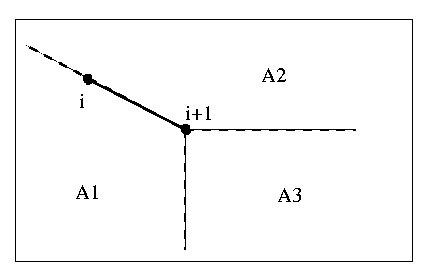
\includegraphics[clip,width=7.0cm]{./img/sklansky2.png}
    \caption{Sklansky法-R1領域の分割}
    \label{fig:sklansky2}
	 {\tiny http://cgm.cs.mcgill.ca/~athens/cs601/}
  \end{center}
\end{figure}

次に頂点I+2を置くことを試みるのだが、条件によってその挙動が決まる。
\begin{enumerate}
\item I+2がR1領域に存在しない場合は、I+2を廃棄する。
\item I+2がA3領域に存在する場合は、I+2を保持し、次の処理に移る。
\item I+2がA2領域に存在するか、
        I+2がA1領域にありかつI+2がI+1の上にあり更に直前の点がこの処理によって廃棄されていた場合は、I+2を廃棄する。
\item I+2がA1領域に存在する場合は、I+1を廃棄する。
\end{enumerate}

(3)の処理を行った場合は、I+2をI+1とし、I+1をIとする。
それ以外の場合はIをひとつ進め、

\end{comment}

凸包から話を戻す。
得られた模様の中で、もっとも面積の大きなものをsizeに代入する。
マッチングを行う際にはこのサイズを基準にするためである。

ここまでで二値化を通して牌の模様の輪郭情報を抽出する処理を行った。
今度はこれをグレースケール画像に適用し、牌一種類ごとのテンプレートを得る。

それにはgridを用いる。
gridはsubmatを実装に含み、元画像から矩形範囲を抽出できる関数である。
gridで牌を4*9に区切り、zipで牌ごとに模様の輪郭の情報を付与し、
それらにflatMapを挟んでgetRectSubPixをかけることによって、
輪郭だけが抽出されたすべての牌のテンプレートを得ることができる。

以上でテンプレートの生成が完了した。

\section{テストデータとの照合}

照合は関数recognizeによって実装されている。
この引数matに手牌の画像データを、templatesにテンプレートの画像データを渡す。

実際に使用した手牌データを図\ref{fig:hand}に示す。

\begin{figure}[H]
  \begin{center}
    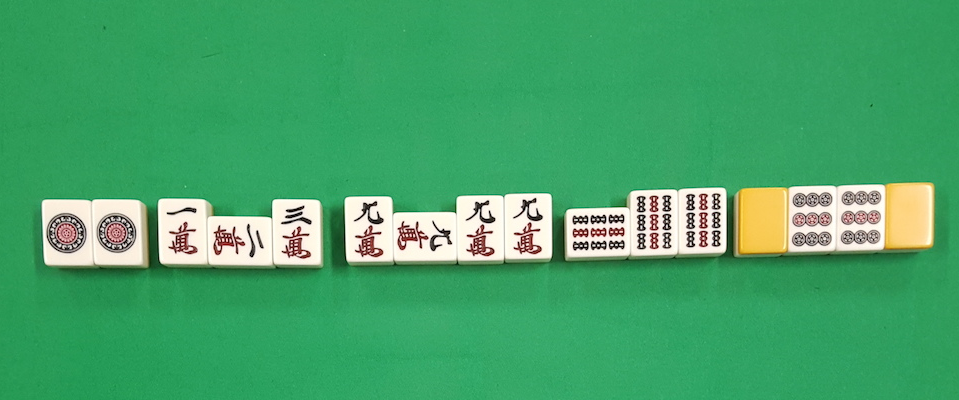
\includegraphics[clip,width=7.0cm]{./img/hand.png}
    \caption{手牌}
    \label{fig:hand}
  \end{center}
\end{figure}

この画像の画素値は幅959x高さ400ピクセルであり、
ビットの深さは32ビットである。
手牌の場合も二値化を施すと8ビットまで圧縮される。

手牌のデータはcropによって背景から切り離される。
しかしテンプレートをcropで切り離したときと違い、
この場合は牌のデータが複数に分かれる。
手牌には純手牌と鳴牌があり、鳴牌は純手牌と離して置くためだ。
この時の出力結果は以下のようになる。

\begin{figure}[H]
  \begin{center}
    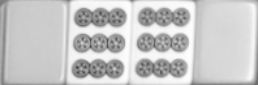
\includegraphics[clip,width=5.0cm]{./img/hand0_0.png}
    \caption{手牌 分離後 1}
    \label{fig:hand0}
    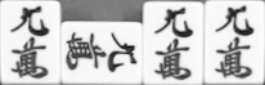
\includegraphics[clip,width=5.0cm]{./img/hand1_0.png}
    \caption{手牌 分離後 2}
    \label{fig:hand1}
    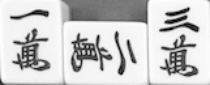
\includegraphics[clip,width=4.0cm]{./img/hand2_0.png}
    \caption{手牌 分離後 3}
    \label{fig:hand2}
    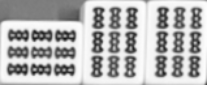
\includegraphics[clip,width=4.0cm]{./img/hand3_0.png}
    \caption{手牌 分離後 4}
    \label{fig:hand3}
    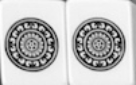
\includegraphics[clip,width=3.0cm]{./img/hand4_0.png}
    \caption{手牌 分離後 5}
    \label{fig:hand4}
  \end{center}
\end{figure}

図のデータの順は、配列変数内の順に一致する。
その順は画像データの面積によって決められており、
分離時に得た輪郭を利用して領域内の面積を求めている。

面積を求めるには、まず輪郭情報から四方向(上下左右)の極地点を取得し、
次に各極値が持つ座標情報から輪郭に外接する矩形を求め、
その長辺と短辺を掛けあわせれば良い。

手牌のデータはcollectによってhandに束縛される。
まずはhandをテンプレートのサイズに合わせてリサイズする。
それから頂点数を求め純手牌か否かの情報をedgeに代入して、
テンプレートに向きを回転させた牌を加えてtilesに代入すると、
いよいよgoでパターンマッチを行う。
	
goの内部では、まず各テンプレートに対してopencvのテンプレートマッチング関数たるmatchTemplateを呼ぶ。
その結果がresultへと代入されるので、
minMaxLocを通して最高スコアと最低スコアの情報を取り出し、
使用したテンプレートとスコア情報のタプルをlocsに加えてゆく。
この手順をすべてのテンプレートに対して実行する。
minMaxLocの返り値はドキュメントによると\cite{minMaxLoc}
Core.MinMaxLocResult型である。
座標を返すmaxLocフィールドと値を返すmaxValフィールドを参照することで最高スコアの情報を得ることができる。

マッチングの結果はは図\ref{fig:result10}のような形で得られる。
結果の画素はテンプレートと比較対象の画素の差であり、白い部分ほどスコアが高いことを意味している。

\begin{figure}[H]
  \begin{center}
    
\includegraphics[clip,width=7.0cm]{./img/matching_result1_0.png}
    \caption{マッチング結果}
    \label{fig:result10}
    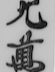
\includegraphics[clip,width=1.0cm]{./img/9wan.png}
    \caption{テンプレート}
    \label{fig:9wan}
  \end{center}
\end{figure}

図\ref{fig:result10}の結果は図\ref{fig:hand1}に対して九萬のテンプレート(図\ref{fig:9wan})でマッチングを行った結果である。
左端と右端、それから「マッチング結果」の「果」の上にあたる部分で白い点のようなものが見えるが、
この三点こそ縦向きの九萬が発見された点を示している。

すべてのテンプレート(及びその回転)に対してのマッチングの結果locsから、
loc値が最大となるものをmaxByによって取得し、変数((tile,loc),i)に代入する。
スコアが最大となる位置はloc.maxLocで参照でき、
それにテンプレートの大きさtile.sizeを組み合わせることで、
マッチした手牌の輪郭rectを得られる。
rectの実装では、最大スコアの場所とサイズから、基準点と縦横のサイズ情報を持つ矩形を作成している。

ここでgoの引数を見てみる。
goの引数はrectsであり、
それはrectと、そのインデックス番号のタプルのシーケンスである。
goは再帰を前提としており、このシーケンスrectsは再帰のたびに認識結果を積み重ねてゆく。

rectangleによってマッチングした牌の輪郭部分に矩形を描き、矩形内部の領域を塗りつぶすと、
goを再帰する。
このときシーケンスである引数rectsにマッチした牌rectを加えており、
rectsはすべての牌についてのマッチングが終了した時には関数goの返り値となる。

矩形を引いた結果を図\ref{fig:rect11}に、塗りつぶした結果を図\ref{fig:hand11}に示す。

\begin{figure}[H]
  \begin{center}
    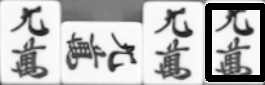
\includegraphics[clip,width=5.0cm]{./img/hand_rect1_1.png}
    \caption{矩形描画}
    \label{fig:rect11}
    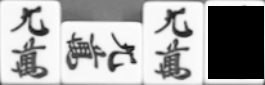
\includegraphics[clip,width=5.0cm]{./img/hand1_1.png}
    \caption{塗りつぶし後}
    \label{fig:hand11}
  \end{center}
\end{figure}

このように塗りつぶされた箇所は、以後の再帰でのマッチングにおいて、
テンプレートにマッチしなくなる。

矩形領域がすべて塗りつぶされたあとは、
適当な地点が最大スコアとして返り、そこからそのループでのrectが得られるが、
intersectsによって現在のrectと過去のrect(rectsに保存)の矩形領域が重なっているか否かの判別を行い、
重なっていた場合にマッチング終了という判定を下す。

マッチングを終えたら結果を手牌の位置順にソートし、シーケンス情報だけを取り出しindicesに代入する。
最後に純手牌か否かの判別を改めて行い、その結果とindicesのタプルをresultに代入していく。

resultは純手牌および鳴牌のまとまり毎に要素数がひとつずつ増える構造であり、
最終的に、純手牌と鳴牌のシーケンスのタプルがrecognizeの返り値となる。

\section{matchTemplateについて}

opencvにおけるテンプレートマッチングを行うメソッドmatchTemplateは、以下の引数を取る。
\begin{enumerate}
\item image,\ テンプレートの探索対象となる画像。8ビットまたは32ビットの浮動小数点型
\item templ,\ 探索されるテンプレート。imageと同じデータ型である必要がある
\item result,\ 比較結果のマップ
\item method,\ 比較方法の指定
\end{enumerate}

プログラムではmethodにTM\_CCORR\_NORMEDを指定している。
これは数式で表すと
\\ \\ 
\begin{figure}[H]
  \begin{center}
    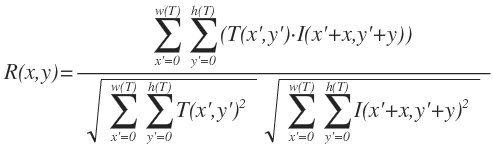
\includegraphics[clip,width=7.0cm]{./img/ccorr.png}
    \caption{相互相関関数}
    \label{fig:ccorr}
  \end{center}
\end{figure}
であり、一般に相互相関関数と呼ばれる式である。
なおw(T)はTの横の画素数を、h(T)はTの縦の画素数を指す。

この式の意味するところは、テンプレートと対象画像の畳込み演算である。
ふたつのベクトル(または関数)に対しての畳込み演算は、
積の総和によって求められる。これを相関と言うが、この値が大きければ大きいほど、正の相関度が高いと言える。

相関について別の見方をすると、ベクトルの内積である。
これを逆手に取って、各ベクトルの大きさの積で割ることによって、
cosθだけを得られるようになる。
$-1\le cos\theta \le 1$より、相関結果にスカラ値の割り算を施すと、-1から1の範囲で正規化される。
相互相関関数の左辺は内積の角度cosθを示しており、
cosθが1に近づけば近づくほど、θは小さく、テンプレートと対象画像の領域が近づいていることを意味する。

各ピクセルに対して内積を求める操作は行われ、その総和を以ってスコアとするので、
スコアが大きければ大きいほど、テンプレートとマッチしているという結果になる。
この点は最小誤差によってマッチングを行うmethodSQDIFFとは逆の意味になっているので、
関数matchTemplateの結果resultには注意が必要である。

matchTemplateの結果であるresultについては、スコアのマップ形式で返される。
マップについて説明する。
そもそもテンプレートマッチングとは、
テンプレート画像と対象画像を重ね合わせて画素の差を比較するという行為を、
各ピクセルに対して行うものである。
つまり重ねあわせが行われる範囲でマッチングの結果が得られるのであって、
それは対象画像のサイズとテンプレート画像のサイズの差の範囲である。
この範囲の行列をマップと呼ぶ。(この呼び名はopencvのドキュメント\cite{matchTemplateC}\cite{matchTemplatePy}に即する)
そしてマップの値にはテンプレートマッチングのスコア(相互相関関数の値)が入るのである。

差の範囲でのみ比較を行うという性質上、テンプレートと対象画像のサイズ差が小さい場合は、
非常に小さい計算量で済むという特徴がある。
テンプレートマッチングの結果である図\ref{fig:result10}を見ると、
横長の帯状の結果が得られているが、
これは図\ref{fig:hand1}の対象画像に対して、図\ref{fig:result10}の範囲のみマッチングを行ったという証左である。

%\begin{lstlisting}[caption=,label=]
%
%\end{lstlisting}

\end{multicols}

\newpage

\begin{thebibliography}{9}
\bibitem{yoshida}
	Sanshiro Yoshida.mahjongs.\\
	https://github.com/halcat0x15a/mahjongs
\bibitem{minMaxLoc}
	OpenCV 2.4.2 Java API.Core.MinMaxLocResult.\\
	http://docs.opencv.org/java/2.4.2/index.html?org/opencv/core/Core.html
\bibitem{matchTemplateC}
	物体検出-opencv2.2 documentation. \\
	http://opencv.jp/opencv-2svn/cpp/object\_detection.html
\bibitem{matchTemplatePy}
	Object Detection-opencv2.4.10.\\
	http://docs.opencv.org/2.4/modules/imgproc/doc/object\_detection.html
\bibitem{contours}
	opencv/contours.cpp-Itseez/opencv. \\
	https://github.com/Itseez/opencv/blob/d8c352d20d2dba96298c26b92b7919e98e47c4c3/modules/imgproc/src/contours.cpp
\bibitem{contoursDoc}
   contours-OpenCV. \\
   http://docs.opencv.org/3.1.0/d4/d73/tutorial\_py\_contours\_begin.html
\end{thebibliography}



\newpage

\section{付録}

\subsection{画像認識}
\begin{lstlisting}[caption=TemplateMatching.scala,label=TemplateMatching]
package mahjongs.recognizer
import org.opencv.core._
import org.opencv.imgproc.Imgproc

object TemplateMatching {

  val MaxResolution: Int = 1024 * 1024

  def createTemplate(mat: Mat): Option[(IndexedSeq[Mat], Size)] = {
    crop(resize(mat, MaxResolution)).headOption.map {
      case (template, _) =>
        val mask = threshold(template.clone, true)
        val width = template.cols / 9
        val height = template.rows / 4
        floodFill(mask, (0 until 4).map(_ * height) :+ (mask.rows - 1), 0 until mask.cols)
        floodFill(mask, 0 until mask.rows, (0 until 9).map(_ * width) :+ (mask.cols - 1))
        Imgproc.dilate(mask, mask, new Mat)
        val rects = for (tiles <- grid(mask, 4, 9)) yield {
          for (tile <- tiles) yield {
            val contours = findContours(tile.clone).flatMap(_.toArray)
            if (contours.length > 0)
              Some(convexHull(contours))
            else
              None
          }
        }
        val size = rects.flatten.flatten.map(_.size).maxBy(_.area)
        val tiles = grid(template, 4, 9).zip(rects).flatMap {
          case (tiles, rects) =>
            tiles.zip(rects).map {
              case (tile, rect) =>
                Imgproc.getRectSubPix(tile, size, rect.fold(center(tile))(center), tile)
                tile
            }
        }.take(34)
        (tiles, new Size(width, height))
    }
  }

  def recognize(mat: Mat, templates: Seq[Mat], width: Int, height: Int): (Seq[Int], Seq[Seq[Int]]) = {
    val result = crop(resize(mat, MaxResolution)).collect {
      case (hand, contour) if hand.size.area > 0 =>
        Imgproc.resize(hand, hand, new Size(hand.size.width * height / hand.size.height, height))
        val edge = approxPoly(new MatOfPoint2f(contour.toArray: _*)).rows
        val tiles = templates ++ templates.map(m => flip(m.t, 0)) ++ templates.map(flip(_, -1)) ++ templates.map(m => flip(m.t, 1))
        def go(rects: List[(Int, Rect)]): List[(Int, Rect)] = {
          val locs = for (tile <- tiles) yield {
            val result = new Mat
            Imgproc.matchTemplate(hand, tile, result, Imgproc.TM_CCORR_NORMED)
            (tile, Core.minMaxLoc(result))
          }
          val ((tile, loc), i) = locs.zipWithIndex.maxBy(_._1._2.maxVal)
          val rect = new Rect(loc.maxLoc, tile.size)
          if (rects.forall(pair => !intersects(rect, pair._2))) {
            Imgproc.rectangle(hand, rect.tl, rect.br, new Scalar(0), -1)
            go((i % 34, rect) :: rects)
          } else {
            rects
          }
        }
        val indices = go(Nil).sortBy(_._2.x).map(_._1)
        (edge == 4 && indices.size != 4, indices)
    }.groupBy(_._1).mapValues(_.map(_._2))
    (result(true)(0), result.get(false).toList.flatten)
  }

}
\end{lstlisting}

\subsection{ユーザ定義関数}
\begin{lstlisting}[caption=package.scala,label=package]
package mahjongs
import scala.collection.JavaConverters._
import scala.collection.mutable.Buffer
import org.opencv.core._
import org.opencv.imgcodecs.Imgcodecs
import org.opencv.imgproc.Imgproc

package object recognizer {

  for {
    ext <- sys.props("os.name").toLowerCase match {
      case name if name.contains("nix") => Some("so")
      case name if name.contains("mac") => Some("dylib")
      case _ => None
    }
  } System.load(getClass.getResource(s"/libopencv_java300.$ext").getPath)

  def findContours(mat: Mat): Buffer[MatOfPoint] = {
    val contours = Buffer.empty[MatOfPoint]
    Imgproc.findContours(mat, contours.asJava, new Mat, Imgproc.RETR_EXTERNAL, Imgproc.CHAIN_APPROX_TC89_KCOS)
    contours.sortBy(Imgproc.contourArea)(Ordering.Double.reverse)
  }

  def floodFill(mat: Mat, rows: Seq[Int], cols: Seq[Int]): Mat = {
    val mask = new Mat
    val color = new Scalar(0)
    for (row <- rows; col <- cols if mat.get(row, col)(0) > 0)
      Imgproc.floodFill(mat, mask, new Point(col, row), color)
    mat
  }

  def grid(mat: Mat, rows: Int, cols: Int): IndexedSeq[IndexedSeq[Mat]] = {
    val height = mat.rows / rows
    val width = mat.cols / cols
    for (row <- 0 until rows) yield {
      val rowRange = new Range(row * height, (row + 1) * height)
      for (col <- 0 until cols) yield
        mat.submat(rowRange, new Range(col * width, (col + 1) * width))
    }
  }

  def approxPoly(contour: MatOfPoint2f, epsilon: Double = 0.01): MatOfPoint2f = {
    val curve = new MatOfPoint2f
    Imgproc.approxPolyDP(contour, curve, Imgproc.arcLength(contour, true) * epsilon, true)
    if (curve.rows % 2 == 0)
      curve
    else
      approxPoly(contour, epsilon + 0.01)
  }

  def threshold(mat: Mat, inv: Boolean): Mat = {
    val (tpe, op) = if (inv) (Imgproc.THRESH_BINARY_INV, Imgproc.MORPH_OPEN) else (Imgproc.THRESH_BINARY, Imgproc.MORPH_CLOSE)
    Imgproc.threshold(mat, mat, 0, 255, tpe | Imgproc.THRESH_OTSU)
    Imgproc.morphologyEx(mat, mat, op, new Mat)
    mat
  }

  def crop(mat: Mat): Buffer[(Mat, MatOfPoint)] = {
    for (contour <- findContours(threshold(mat.clone, false))) yield {
      val patch = new Mat
      val rect = Imgproc.minAreaRect(new MatOfPoint2f(contour.toArray: _*))
      Imgproc.warpAffine(mat, patch, Imgproc.getRotationMatrix2D(rect.center, rect.angle, 1), mat.size)
      Imgproc.getRectSubPix(patch, rect.size, rect.center, patch)
      if (rect.angle <= -45) Core.flip(patch.t, patch, 0)
      (patch, contour)
    }
  }

  def convexHull(contours: Seq[Point]): Rect = {
    val hull = new MatOfInt
    Imgproc.convexHull(new MatOfPoint(contours: _*), hull, false)
    Imgproc.boundingRect(new MatOfPoint(hull.toArray.map(contours): _*))
  }

  def flip(mat: Mat, code: Int): Mat = {
    val m = new Mat
    Core.flip(mat, m, code)
    m
  }

  def resize(mat: Mat, max: Int): Mat = {
    val r = math.sqrt(mat.rows * mat.cols / max.toDouble)
    if (r > 1) Imgproc.resize(mat, mat, new Size(mat.size.width / r, mat.size.height / r))
    mat
  }

  def center(mat: Mat): Point =
    new Point(mat.size.width / 2, mat.size.height / 2)

  def center(rect: Rect): Point =
    new Point(rect.x + rect.width / 2, rect.y + rect.height / 2)

  def toMat(bytes: Array[Byte], gray: Boolean): Mat =
    Imgcodecs.imdecode(new MatOfByte(bytes: _*), if (gray) Imgcodecs.CV_LOAD_IMAGE_GRAYSCALE else Imgcodecs.CV_LOAD_IMAGE_COLOR)

  def fromMat(mat: Mat): Array[Byte] = {
    val buf = new MatOfByte
    Imgcodecs.imencode(".png", mat, buf)
    buf.toArray
  }

  def intersects(a: Rect, b: Rect): Boolean =
    math.max(a.x, b.x) < math.min(a.x + a.width, b.x + b.width) && math.max(a.y, b.y) < math.min(a.y + a.height, b.y + b.height)

  def read(filename: String, gray: Boolean): Mat =
    Imgcodecs.imread(filename, if (gray) Imgcodecs.IMREAD_GRAYSCALE else Imgcodecs.IMREAD_COLOR)

}
\end{lstlisting}

\end{document}